
\chapter{Hidden variables for semiclassical models with state-dependent forces}

Define/describe what a hidden variable theory is, drawing heavily on Aaronson's~\cite{Aaronson2005} explanations. Give examples, argue why the Schrodinger theory is appealing.

Motivate with Stern-Gerlach experiment, and derive the method, show what sorts of problems it
solves and where it disagrees with other models, provide simulation results. Limitations: no time dependent potentials, no 3D.

Possibly include speculation about these:

Maybe include a test to see whether it actually does work in 3D as-is, since we haven't actually checked, we just haven't been able to show on paper that current behavior is correct in 3D (also haven't shown it's incorrect).

Time dependent potentials could potentially be handled by approximating unitary as product of part due to spatial variation in H, and part due to time variation in H. compute transition probs for both such that a transition can be attributed to one or the other - only do velocity jumps to conserve potential if due to spatial motion, as time dependent potential can exchange energy with particle.

Matrix scaling for Schrodinger theory, discuss methods: Sinkhorn-Knopp, Lineal, and my one. Compare time complexity of algorithms so as to define the computational complexity of the hidden variables semiclassical method. Method is of course parallelisable on GPU or similar so is fast on parallel machines even if matrix scaling is slow.

Discuss how it would make sense for the systems to behave in the presence of collisions w.r.t collapse of state vectors.

\section{Approximate Markovian decoherence rate for separating wavepackets}

Positional separation of two different internal states of an atom leads to decoherence of those states, with a decoherence factor $r_{ij}(t)$ equal to the overlap of the spatial wavefunctions of the two components in question a time $t$ after they began separating. Approximating both wavepackets as initially overlapping Gaussians of width $\sigma$, ignoring dispersion, and assuming they separate with constant relative acceleration $a_{ij}$, the decoherence factor is

\begin{align}
r_{ij}(t) &= \braket{\psi_i(t)}{\psi_j(t)}\\
 &= C \int_{-\infty}^{\infty} e^{-\frac{x^2}{4\sigma^2}}e^{-\frac{(x-x_\up{rel})^2}{4\sigma^2} + ik_\up{rel}x}\,\dd x,\label{eq:gaussian_integral}
\end{align}
where
\begin{align}
x_{\mathrm{rel}}(t) = \frac12a_{ij}t^2
\end{align}
and
\begin{align}
k_\up{rel}(t) = \frac m \hbar a_{ij} t
\end{align}
are the wavepackets' relative\footnote{$a_{ij}$, $x_\up{rel}$ and $k_\up{rel}$ are the acceleration, position, and wavenumber of the $j^\up{th}$ component with respect to the $i^\up{th}$ component, that is, $a_{ij} = a_j - a_i$, etc.} position and wavenumber due to acceleration for a time $t$ starting from zero relative velocity, and
\begin{align}
C^{-1}=\int_{-\infty}^\infty e^{-\frac{x^2}{2\sigma^2}}\,\dd x\label{supp:eq:Cdef}
\end{align}
is a normalisation constant [TODO CHECK IF NEEDS TO BE SQUARED]. Note that this expression holds for any number of dimensions---relative motion is only along one axis so the integrals in all other directions equal one.

Evaluating the Gaussian integral \eqref{eq:gaussian_integral} gives the following expression for the decoherence factor $r_{ij}(t)$:
\begin{align}
r_{ij}(t)&= e^{-\left[
        \frac{1} {8\sigma^2} x_\up{rel}^2
      + \frac i2 x_{\mathrm{rel}} k_\up{rel}
      + \frac{\sigma^2}{2} k_\up{rel}^2
      \right]}\label{eq:decoherence_factor}.
\end{align}

This is a decoherence \emph{factor}; it is the factor by which the $(i, j)$ off-diagonal of the reduced density matrix for the atom's internal state will be reduced at time $t$. The corresponding decoherence \emph{rate} is given by the logarithmic derivative of \eqref{eq:decoherence_factor}:

\begin{align}
\Gamma_{ij}(t) = - \frac 1 {r_{ij}(t)} \dv t {r_{ij}(t)}.
\end{align}

 The fact that \eqref{eq:decoherence_factor} does not describe a constant decoherence rate (i.e., it does not have the functional form of exponential decay) means that the back-action on the atom's internal state caused by measurements of its motional state will be different depending on the interval of time between measurements.

For example, the logarithmic derivative of \eqref{eq:decoherence_factor} approaches zero as $t$ goes to zero. This means that in the limit of infinitely frequent measurements, no decoherence occurs at all in between measurements, and the motional state is reset after each measurement such that the wavepackets never separate at all. This is the quantum Zeno effect, and its appearance in models of open quantum systems is usually treated as a reminder that the assumption of infinitely frequent strong measurements is unphysical [CITE].

Since experimentally we are not measuring atoms' motional states so frequently, we ought to wait until the wavepackets are completely separated before performing a projective measurement. As in quantum optics models of open quantum systems, in which the measurement interval ``should be large enough to allow the photons to get away from the atom" [CITE The Quantum Jump Approach
and Quantum Trajectories Gerhard C. Hegerfeldt], ours should be large enough for the atomic states to get away from each other.

If at large enough times, a decoherence rate is independent of time, that decoherence is called Markovian at that timescale. A Markovian environment is one that has no memory of the decoherence process---it ``forgets" any information caused by past interaction with the system. Even though at short times, all decoherence rates in quantum mechanics tend to zero [CITE], if they become Markovian on a timescale shorter than other timescales of interest, the Markov approximation can be used and a constant decoherence rate used at all times. In quantum optics, the decoherence factor for the internal state of an atom due to photon emission indeed tends to exponential decay on timescales that are still much shorter than that of the system evolution, and thus the Markov approximation is accurate.

Unlike quantum optics models, our decoherence factor does not describe Markovian decoherence on any timescale. In the limit of large $t$, its functional form is $e^{-t^4}$, not the exponential decay required to treat the decoherence as Markovian [CITE] at that timescale. Nonetheless, if we wish to write a time-local differential equation for the internal state of the atom, Markovian decoherence is the only kind we can include [CITE].

To that end, we will now construct a ``time ignorant" version of $r_{ij}(t)$ that answers the question ``What is the expected decoherence factor at all future times, if you don't know how long it has been since the two wavepackets began separating?" In this way we can compute an \emph{average} decoherence rate $\Gamma_{ij}$ described by our decoherence factor, even though $r_{ij}(t)$ does not have a constant decoherence rate at large times. This essentually amounts to finding the best fitting exponential to $r_{ij}(t)$. Whilst this approximation is crude, it is nonetheless an improvement over the Ehrenfest model, which has no decoherence at all (i.e. it has a decoherence rate that is also constant like ours---but equal to zero).

\begin{figure}[t]
    \centerfloat
    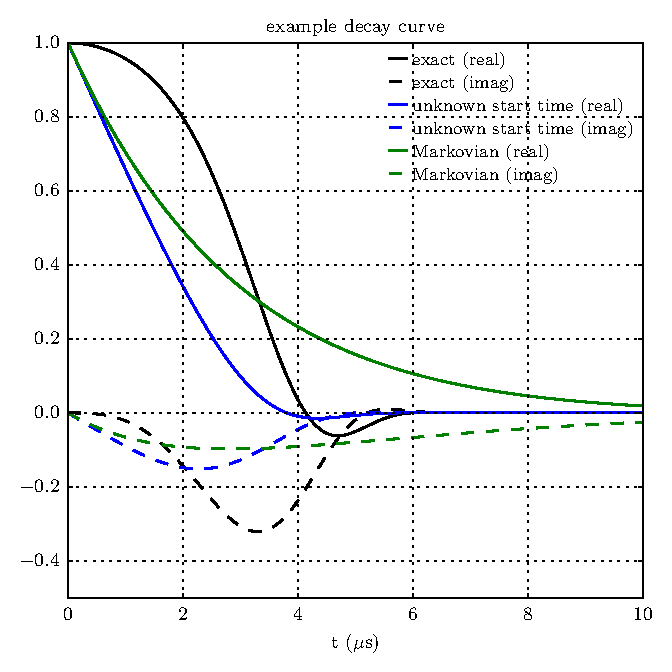
\includegraphics{figures/hidden_variables/decoherence_factor_example.pdf}
    \caption{Caption.}
    \label{fig:decoherence_factor_example}
\end{figure}

We define the time-ignorant decoherence factor $\tilde r_{ij}(t)$ as the overlap of the wavefunction of the $i^\up{th}$ internal state with a superposition of wavepackets of the $j^\up{th}$ internal state, with the superposition being over all times in the past the wavepackets began separating:
\begin{align}
\tilde r_{ij}(t) &= \bra{\psi_i(t)} A\int_{-\infty}^0 \ket{\psi_j(t - t^\prime)} \,\dd t^\prime,
\end{align}
where $A$ is a normalisation constant such that $\tilde r_{ij}(0) = 1$.
Since $\ket{\psi_i(t)}$ is time independent (rather, since we can perform our calculations in the frame of reference in which it is stationary), this is:
\begin{align}
\tilde r_{ij}(t) &= A\int_{-\infty}^0 r_{ij}(t - t^\prime) \,\dd t^\prime,
\end{align}
which is simply the convolution of our decoherence factor with a step function which is nonzero at all negative times.
Our average decoherence rate $\Gamma_{ij}$ is then given by the logarithmic derivative of $\tilde r_{ij}(t)$ at $t=0$:

\begin{align}
\Gamma_{ij} &= -\frac {\tilde r_{ij}^\prime(0)} {\tilde r_{ij}(0)}\\
&= -\frac {\int_0^\infty \tilde r_{ij}^\prime(t)\,\dd t} {\int_0^\infty \tilde r_{ij}(t)\, \dd t}\\
\Rightarrow \Gamma_{ij}^{-1}&= \int_0^\infty e^{-\left[
        \frac{1} {8\sigma^2} x_\up{rel}^2
      + \frac i2 x_{\mathrm{rel}} k_\up{rel}
      + \frac{\sigma^2}{2} k_\up{rel}^2
      \right]}\, \dd t.\label{eq:gamma_integral}
\end{align}

As mentioned, $\Gamma_{ij}$ is the decay constant for the best fitting exponential to our decoherence factor \eqref{eq:decoherence_factor}. Although \eqref{eq:decoherence_factor} looks nothing like a decaying exponential in time, an exponential approximation to it nonetheless ought to decay to zero on the same timescale. An example of this is shown in \figref{fig:decoherence_factor_example}

In order to obtain an approximate analytic expression for this integral, we consider two limiting cases and then stitch them together in the intermediate regime. In the limit of small wavepackets, $\sigma$ is small and thus the first term in the exponent in \eqref{eq:gamma_integral} is largest, and the third term is smallest. In this regime, which describes when positional separation (as opposed to separation in $k$-space) dominates the decoherence, we'll neglect the third term in the exponent and treat the second term as small relative to the first.
This gives us:
\begin{align}
\Gamma_{ij\,\up{(pos)}}^{-1} &\approx \int_0^\infty e^{-\left[
        \frac{1} {8\sigma^2} x_\up{rel}^2
      + \frac i2 x_{\mathrm{rel}} k_\up{rel}
      \right]}\, \dd t.\\
      &\approx \int_0^\infty e^{-
              \frac{1} {8\sigma^2} x_\up{rel}^2}\left(1 - \frac i2 x_{\mathrm{rel}} k_\up{rel}\right)\, \dd t.\label{eq:gamma_pos_exp}\\
      &= 2^{\frac54}\upGamma(\tfrac54)\sqrt{\frac{\sigma}{a_{ij}}} - 2i\frac{m \sigma^2}{\hbar},\label{eq:gamma_pos_recip}
\end{align}
where we used a first-order Taylor expansion of an exponential in \eqref{eq:gamma_pos_exp}. We similarly use a first order expansion to take the reciprocal of \eqref{eq:gamma_pos_recip} (since the second term is much smaller than the first\footnote{This isn't necessary in order to obtain a simple expression for $\Gamma_{ij\,\up{(pos)}}$---the reciprocal without this approximation is equally simple---but it leaves us with power laws for the real and imaginary parts of $\Gamma_{ij\,\up{(pos)}}$, which are easier to stitch together with those from the large $\sigma$ regime.}), and arrive at:
\begin{align}
\Gamma_{ij\,\up{(pos)}} &\approx \frac1{2^{\frac54}\upGamma(\tfrac54)}\sqrt{\frac{a_{ij}}{\sigma}}
+ \frac i {2\sqrt{2}\upGamma(\tfrac54)^2} \frac{m\sigma a_{ij}}{\hbar}\label{eq:gamma_pos_final}%\\
% &\approx 0.463865\sqrt{\frac{a_{ij}}{\sigma}}
% + 0.430341 i \frac{m\sigma a_{ij}}{\hbar}.
\end{align}

Similarly for the large $\sigma$ regime, we neglect the first term in the exponent of \eqref{eq:gamma_integral} and consider the second term small relative to the third. This is the regime in which the decrease in overlap of the two wavepackets is dominated by their separation in velocity space. Following the same process as above gives:
\begin{align}
\Gamma_{ij\,\up{(vel)}}^{-1} &\approx \int_0^\infty e^{-\left[
        \frac i2 x_{\mathrm{rel}} k_\up{rel}
        + \frac{\sigma^2}{2} k_\up{rel}^2
      \right]}\, \dd t.\\
      &\approx \int_0^\infty \left(1 - \frac i2 x_{\mathrm{rel}} k_\up{rel}\right)
      e^{-\frac{\sigma^2}{2} k_\up{rel}^2}\, \dd t\\
      & = \sqrt{\frac\pi2}\frac\hbar{m \sigma a_{ij}} - i\frac{\hbar^3}{2m^3 \sigma^4 a_{ij}^2}\\
      \Rightarrow \Gamma_{ij\,\up{(vel)}} &\approx \sqrt{\frac2\pi}\frac{m \sigma a_{ij}}\hbar
                                          + \frac i\pi \frac\hbar{m \sigma^2}
                                          \label{eq:gamma_vel_final}
\end{align}
Equations \eqref{eq:gamma_pos_final} and \eqref{eq:gamma_vel_final} are our final expressions for the docoherence rate in the limit of small and large wavepackets respectively. Adding their real parts in quadrature and adding the reciprocals of their imaginary parts then provides a reasonable approximation for $\Gamma_{ij}$ over all wavepacket sizes:
\begin{align}
\Gamma_{ij} \approx
\left[\re(\Gamma_{ij\,\up{(pos)}})^2 + \re(\Gamma_{ij\,\up{(vel)}})^2\right]^{\frac12}
+ i\left[\im(\Gamma_{ij\,\up{(pos)}})^{-1} + \im(\Gamma_{ij\,\up{(vel)}})^{-1}\right]^{-1}.
\label{eq:gamma_total}
\end{align}

\begin{figure}[t]
    \centerfloat
    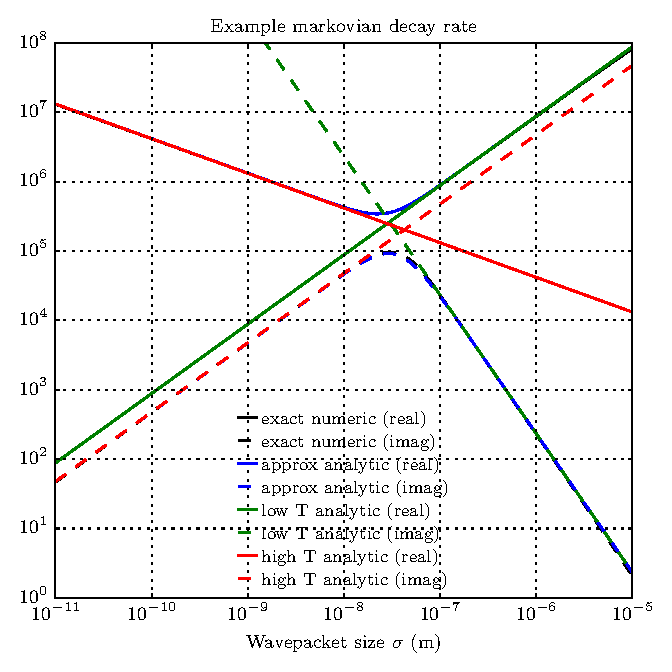
\includegraphics{figures/hidden_variables/decoherence_rate_example.pdf}
    \caption{Caption.}
    \label{fig:decoherence_rate_example}
\end{figure}

We now have an approximate analytic expression that not computationally inexpensive to evaluate for each atom in an ensemble at every timestep of a differential equation.
An example showing the accuracy of \eqref{eq:gamma_total}, compared to the exact expression \eqref{eq:gamma_integral} for for $\Gamma_{ij}$ over a range of wavepacket sizes is shown in \figref{fig:decoherence_rate_example}.

\section{Choice of wavepacket size}

How big is a wavepacket?
